
\documentclass[9pt]{beamer}
%\makeatletter
%\def\beamer@calltheme#1#2#3{%
%	\def\beamer@themelist{#2}
%	\@for\beamer@themename:=\beamer@themelist\do
%	{\usepackage[{#1}]{\beamer@themelocation/#3\beamer@themename}}}
%
%\def\usefolder#1{
%	\def\beamer@themelocation{#1}
%}
%\def\beamer@themelocation{}

%\usefolder{../config}

\usetheme[
block=fill,
titleformat=regular,
progressbar=frametitle
]{metropolis}
%\metroset[everytitleformat=regular] % regular, lowercase, uppercase ]
%\metroset[inner/block=fill]

%\setbeameroption{show notes} 
\usepackage{booktabs}
\usepackage[scale=2]{ccicons}

\usepackage{pgfplots}
\usepgfplotslibrary{dateplot}


%\ Hrvatski znakovi
\usepackage[utf8]{inputenc}
\usepackage[T1]{fontenc}
\usepackage[croatian]{babel}
\usepackage{todonotes}
\usepackage{amsmath}
\usepackage{amsfonts}
\selectlanguage{croatian} % american ngerman
\usepackage{todonotes}

% Koristenje Latin modern fonta
% Bez toga na nekim racunalima baca
% err: Font <taj i taj> at <mala velicina, npr4.0pt> not loadable: Metric (TFM) file not found. \end{frame}
\usepackage{lmodern}


\definecolor{RoyalBlue}{cmyk}{1, 0.50, 0, 0}
%\usepackage{natbib}
%\usepackage{bibentry}
\usepackage{scrextend}
\usepackage{hyperref}
%\usepackage[pdfa=true]{hyperref}
\hypersetup{%
    %draft, % = no hyperlinking at all (useful in b/w printouts)
    %colorlinks=true, 
    linktocpage=true, pdfstartpage=3, pdfstartview=FitV,%
    % uncomment the following line if you want to have black links (e.g., for printing)
    %colorlinks=false, linktocpage=false, pdfborder={0 0 0}, pdfstartpage=3, pdfstartview=FitV,% 
    breaklinks=true, pdfpagemode=UseNone, pageanchor=true, pdfpagemode=UseOutlines,%
    plainpages=false, bookmarksnumbered, bookmarksopen=true, bookmarksopenlevel=1,%
    hypertexnames=true, pdfhighlight=/O,%nesting=true,%frenchlinks,%
    %urlcolor=webbrown, linkcolor=RoyalBlue, citecolor=webgreen, %pagecolor=RoyalBlue,%
    %urlcolor=Blue, linkcolor=Blue, citecolor=Red, %pagecolor=Black,%
    %pdftitle={\myTitle},%
    %pdfauthor={\textcopyright\ \myName, \myUni, \myFaculty},%
    pdfsubject={},%
    pdfkeywords={},%
    pdfcreator={pdfLaTeX},%
    pdfproducer={LaTeX with hyperref and classicthesis}, %
    unicode = true 
} 

%\usepackage[pdftex]{graphicx}
% declare the path(s) where your graphic files are
\graphicspath{{./}{./figures/}}


\newcommand{\executeiffilenewer}[3]{%
	\ifnum\pdfstrcmp{\pdffilemoddate{#1}}%
	{\pdffilemoddate{#2}}>0%
	{\immediate\write18{#3}}\fi%
}
\newcommand{\includesvg}[1]{%
	\executeiffilenewer{#1.svg}{#1.pdf}%
	{inkscape -z -C --file=#1.svg %
		--export-pdf=#1.pdf --export-latex}%
	\input{#1.pdf_tex}%
}


% http://tex.stackexchange.com/questions/83882/how-to-highlight-python-syntax-in-latex-listings-lstinputlistings-command

\usepackage{listings}
\usepackage{color}
\usepackage[semibold]{sourcecodepro}

% Default fixed font does not support bold face
\DeclareFixedFont{\ttb}{T1}{txtt}{bx}{n}{12} % for bold
\DeclareFixedFont{\ttm}{T1}{txtt}{m}{n}{12}  % for normal
% Custom colors
\definecolor{deepblue}{rgb}{0,0,0.5}
\definecolor{deepred}{rgb}{0.6,0,0}
\definecolor{deepgreen}{rgb}{0,0.5,0}


% Python style for highlighting
\newcommand\pythonstyle{\lstset{
		language=Python,
		basicstyle=\small\ttfamily,
		otherkeywords={self},             % Add keywords here
		keywordstyle=\small\ttfamily\color{deepblue},
		emph={MyClass,__init__},          % Custom highlighting
		emphstyle=\small\ttfamily\color{deepred},    % Custom highlighting style
		stringstyle=\color{deepgreen},
		frame=tb,                         % Any extra options here
		showstringspaces=false            % 
	}}
	
	
	% Python environment
	\lstnewenvironment{python}[1][]
	{
		\pythonstyle
		\lstset{#1}
	}
	{}
	
	% Python for external files
	\newcommand\pythonexternal[2][]{{
			\pythonstyle
			\lstinputlisting[#1]{#2}}}
	
	% Python for inline
	\newcommand\pythoninline[1]{{\pythonstyle\lstinline!#1!}}
%\documentclass[ucs]{beamer}
%\usetheme[menuwidth={0.3\paperwidth}]{erlangen}
%\setbeamercovered{transparent=20} 

\usepackage{amsmath,amsfonts,amsthm,amssymb}
\usepackage{setspace}
\usepackage{Tabbing}
\usepackage{fancyhdr}
\usepackage{lastpage}
\usepackage{extramarks}
\usepackage{chngpage}
\usepackage{soul,color}
\usepackage{graphicx,float,wrapfig}
\usepackage{xcolor}
\usepackage[normalem]{ulem}
\usepackage{mathtools}

\definecolor{erlangenlyellow}{RGB}{123, 25, 121}
%\usepackage[utf8x]{inputenc}
%\usepackage{default}
%\usepackage[T1]{fontenc}

\usepackage{verbatim}
\usepackage{listings}


\usepackage{subcaption}
\usepackage{lmodern}

\title{Uvod}

\subtitle{how Occam would be ashamed}
\institute{Računalna grafika}


\begin{document}
\begin{frame}
 \titlepage
\end{frame}

%\begin{frame}{Sadržaj}
%  \tableofcontents
%  % You might wish to add the option [pausesections]
%\end{frame}
\section{Obveze}
\begin{frame}
	\begin{itemize}
		\item Tijekom semestra je moguće dobiti najviše 70 bodova, kao i na završnom ispitu.
		\item Obveze: Uspješno položena dva kolokvija i jedna domaća zadaća.
	\end{itemize}
\end{frame}
\begin{frame}{Domaća zadaća}
	\begin{itemize}
		\item Domaća zadaća iznosi $K_{dz} = 20$ bodova. 
		\item Najmanji broj bodova za koje se smatra da je student/ica uspješno izvršila svoj zadatak iznosi $K_{dz} = 11$ bodova. 
		\item Ako se ostvari $K_{dz}<11$ bodova, onda se zahtijeva da ispravi kod toliko da ostvari najmanje $11$ bodova, ili, $K_{dz}\ge 11 $. 
		\begin{itemize}
			\item btw, to se rijetko dešava.
		\end{itemize}
		\item Nužan, ali ne i dovoljan uvjet: program mora koliko-toliko riješiti zadani zadatak.
	\end{itemize}
\begin{center}
	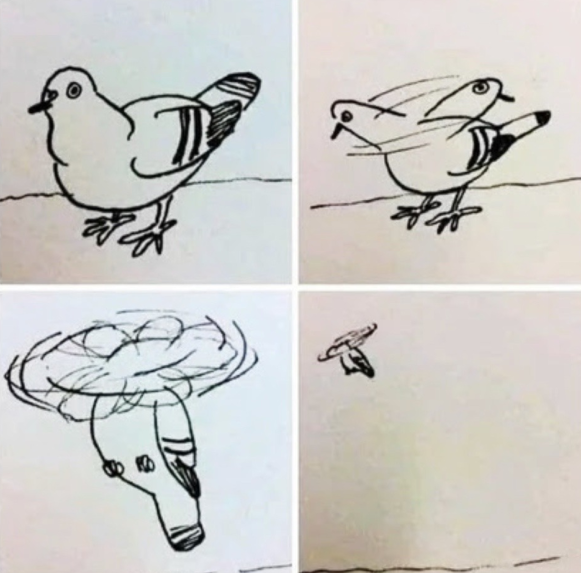
\includegraphics[height=3cm]{./slike/programming_meme_bird.png}
	
\includegraphics[height=3cm]{./slike/pole_screws.jpg}
\end{center}
\end{frame}
\begin{frame}{Kolokviji}
	\begin{itemize}
		\item Svaki kolokvij iznosi $K_k = 25$ bodova. 
		\item Najmanji broj bodova za koje se smatra da je student/ica uspješno položila kolokvij iznosi $K_k = 12$ bodova, odnosno najviše $50$ i minimalno $24$ bodova iz oba kolokvija.
		\item Ako se na jednom ili oba kolokvija dobije manje od $K_k < 12$ bodova, piše se popravni kolokvij koji obuhvaća gradivo oba kolokvija i bodovno iznosi najviše $50$ bodova.
	\end{itemize}
\end{frame}

\begin{frame}{Konačno, bodovi}
	\begin{itemize}
		\item Ukupan broj bodova tijekom semestra Ks računa se prema izrazu:
	\end{itemize}
	\begin{align*}
	K_s = K_{dz}+ K_k
	\end{align*}

gdje je $K_{dz}$ broj bodova domaće zadaće, a $K_k$ broj bodova na kolokvijima. 
\\\hrulefill\\
Kolokviji, 
	\begin{align*}
		\textrm{if}&&  K_1>=12\  \mathtt{and}  \ K_2>=12 &:&          K_k = K_1 + K_2 \\
		\textrm{else}&&   &&          K_k = \frac{K_1+K_2 + K_p}{2}
	\end{align*}
Ovdje su $K_1$ i $K_2$ broj bodova na 1. odnosno 2. kolokviju, a $K_p$ broj bodova na popravnom kolokviju.

\end{frame}


\begin{frame}{Bodovi tldr;}
	\begin{block}{}
		\begin{itemize}
			\item Minimalni broj bodova: dz 11, kolokviji 12 bodova. 
			\item Ako  je jedan ili oba kolokvija <12, piše se jedan popravni kolokvij koji obuhvaća oba kolokvija. 
			\item Ukupna ocjena iz kolokvija je srednja vrijednost oba kolokvija i popravnog kolokvija. 
			\item Ako je dz <11, onda tražim da ispravite kod i predate opet.  
		\end{itemize}
	\end{block}
\end{frame}
\section{O kolegiju}
\begin{frame}
	\begin{columns}[t]
		
		
		\begin{column}{0.4 \textwidth}
			\textbf{Predavanja}
				\begin{itemize}
				\item Osnovni koncepti/algoritmi/tehnike
				\item Interpolacije
				\item Geometrijske transformacije
				\item Krivulje i plohe
				\item Strukture podataka
				\item Svjetlo, boje, materijali i sjene
				\item Ray tracing
			\end{itemize}
		\end{column}

		
		\begin{column}{0.4 \textwidth}
			\textbf{Vježbe}
		\begin{itemize}
			\item C++17
			\item CMake
			\item OpenGL
			\item GLFW, GLEW, glm, glsl
			\item Preferiram Linux, ali ok su i Windows-i
		\end{itemize}
	\end{column}
	\end{columns}
\end{frame}

\begin{frame}{Literatura}
	\begin{itemize}
		\item Čupić M. i Mihajlović Ž. ; \textit{Interaktivna računalna grafika kroz primjere u OpenGL-u}
		\item Marschner S., Shirley P.; \textit{Fundamentals of Computer Graphics}, 4. izdanje, 2016
	\end{itemize}
\end{frame}
\plain{Pitanja?}
\end{document}